\chapter{General Context Of The Project}
This project serves the purpose of developing a platform to manage coding
events,

\section{Introduction}
In the course of this first chapter, I will examine the host organization, its
history, and its organizational chart. Then, I will explore the project's
context, the issues raised, and a technical analysis of the proposed solution.
Finally, I will determine the method to follow to successfully carry out my
project.

\section{Host company}
Orange Digital Center\cite{OrangeDigitalCenter} is a technological center that
is accessible and totally
free
that offers a wide range of trainings, workshops, and events to the community
of the
youth developers, geeks et people who have ideas and projects. In particular,
it addresses
students, entrepreneurs, developers, and graduates.

\begin{figure}[h]
      \centering
      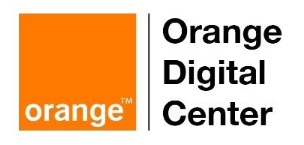
\includegraphics[width=0.5\textwidth]{images/odc.png}
      \caption{Orange Digital Center Logo}
      \label{fig:Orange Digital Center Logo}
\end{figure}

\subsection{Area of expertise}

\subsection{Organization chart}

\subsection{History of the company}
In 2010, Orange Digital Center began its journey in Tunisia, initially focusing
on training young students in new technologies. Over time, this initiative
evolved into a significant network, expanding its influence across various
African countries. Currently, the ODC plays a crucial role in enhancing digital
skills and promoting innovative entrepreneurship in Africa. Thanks to its
successes and growing influence, the Orange Digital Center continues to play a
vital role in the region's digital transition, providing new opportunities for
young talents and future innovators
\subsection{Services}
Orange Digital Center offers a wide range of services to satisfy the needs of
the youth community of developers and entrepreneurs. These services include:

\begin{itemize}
      \item \textbf{Code School:} A technological center providing training
            and activities aimed at enhancing programming and technology
            skills.
      \item \textbf{Solidarity FabLab:} A space offering users an environment
            equipped with digital machines and tools that allow them to
            design prototypes
            and experiment with various projects concretely.
      \item \textbf{Orange Fab:} A startup accelerator providing personalized
            support to young companies, thus fostering the creation of
            national and
            international business partnerships with various entities of the
            Orange group.
      \item \textbf{Orange Ventures:} An investment initiative worth 350
            million euros, with a global scope, providing financial support
            to innovative
            startups in various technological fields, in line with Orange's
            areas of
            expertise.
\end{itemize}

\section{Project Context}
This project aims to develop a platform to host online coding events and
evaluate job candidates by testing their problem solving skills. The goal
is to provide a user-friendly interface and a seamless experience for ODC
coordinators, candidates and event participants.

\subsection{Problematic}
the Orange Digital Center lacks a dedicated platform to
manage coding events and evaluate job candidates. This leads to several
challenges, including:
\begin{itemize}
      \item Difficulty in tracking candidates and managing internships
            applications
      \item Lack of a centralized platform for event management
      \item No KPIs to evaluate the engagement and performance of candidates
\end{itemize}

\subsection{Analysis of the current situation}
most of the existing platforms in the market either comes with a high cost or
lack the flexibility to adapt to the specific needs of the Orange Digital
Center, thus
necessitating the development of a custom solution. The proposed platform will
address the existing challenges and provide a comprehensive solution for event
management, candidate evaluation, and internship tracking.

\subsection{Solution}
The proposed solution is to develop a custom platform that will serve as a
centralized hub for managing coding events, tracking candidates, and evaluating
internship applications. The platform will feature user-friendly interfaces for
ODC coordinators, candidates, and event participants, enabling seamless
interaction and efficient management of the entire process.

\section{Methodology}
In this section, we discuss the methodology employed in our project.
Methodology outlines the approach, techniques, and frameworks utilized to guide
the project's execution and achieve its objectives efficiently. For our
internship project, we embraced Agile methodology, particularly focusing on the
Scrum framework. This section provides an overview of Agile principles,
followed by an in-depth exploration of Scrum, including its definition and key
roles within the framework.

\subsection{Agile Methodology}

Agile methodology is an iterative approach to software development that
prioritizes flexibility, customer collaboration, and incremental delivery. It
emphasizes adaptive planning, evolutionary development, early delivery, and
continuous improvement.

\subsection{Scrum Framework}

Scrum is a popular Agile framework for managing complex software development
projects. It is characterized by its iterative and incremental nature, with a
focus on delivering high-quality products efficiently.

\begin{figure}
      \centering
      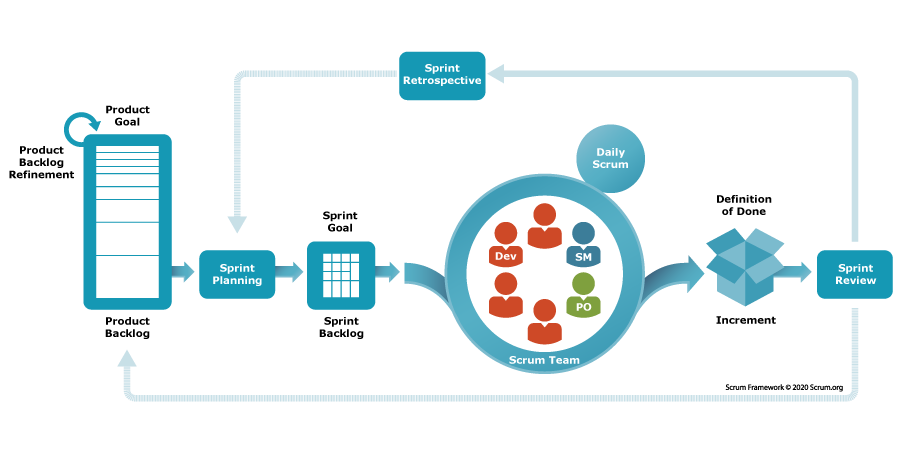
\includegraphics[width=1\textwidth]{images/scrum.png}
      \caption{Scrum Framework}
      \label{fig:Scrum Framework}
\end{figure}

\subsubsection{What is Scrum}

Scrum is a lightweight Agile framework that provides a structured yet flexible
approach to software development. It emphasizes teamwork, transparency, and
frequent inspection and adaptation. Scrum is based on a set of values,
principles, and practices that guide the development process.

\subsubsection{Roles in Scrum}

In Scrum, there are three primary roles:

\begin{itemize}[label=]
      \item \textbf{Product Owner:} The Product Owner is responsible for
            defining and prioritizing the product backlog, representing the
            interests of
            the stakeholders, and ensuring that the team delivers value to
            the customer.
      \item \textbf{Scrum Master:} The Scrum Master is a servant-leader who
            facilitates the Scrum process, removes impediments, and helps the
            team work
            together effectively. They also coach the team on Agile practices
            and
            principles.
      \item \textbf{Development Team:} The Development Team is a
            self-organizing, cross-functional group responsible for
            delivering a
            potentially shippable product increment at the end of each
            sprint. They
            collaborate closely to design, develop, and test the product.
\end{itemize}

\subsection{UML Modeling}

UML (Unified Modeling Language) is a standardized general-purpose modeling
language in the field of software engineering. It provides a set of graphical
notation techniques to create visual models of software-intensive systems. UML
helps to specify, visualize, construct, and document the artifacts of a
software system.

\subsubsection{What is UML}

Unified Modeling Language (UML) is a visual language used to model software
systems. It offers a standardized way to represent the structure, behavior, and
interactions of software components, making it easier for stakeholders to
understand, communicate, and collaborate on software development projects. UML
diagrams can range from high-level conceptual models to detailed designs,
covering aspects such as classes, objects, relationships, activities, and
states.

\subsubsection{Why UML}

UML is widely adopted in the software development industry for several reasons:

\begin{itemize}[label=-]
      \item \textbf{Standardization:} UML is an industry-standard modeling
            language, endorsed by the Object Management Group (OMG), providing
            a
            common
            language and notation for software development.
      \item \textbf{Communication:} UML diagrams serve as a visual
            communication
            tool, enabling stakeholders to convey complex software concepts in
            a
            clear and
            concise manner.
      \item \textbf{Analysis and Design:} UML facilitates the analysis and
            design
            of software systems by capturing requirements, defining
            architecture,
            and
            specifying detailed designs through various types of diagrams.
      \item \textbf{Visualization:} UML diagrams help developers visualize the
            structure, behavior, and interactions of software components,
            aiding in
            understanding and decision-making during the development process.
\end{itemize}

\section{Conclusion}
In this initial section, we introduced the Orange Digital Center, a major
technological hub in Africa, along with its origins and offerings aimed at
young developers and entrepreneurs. We also emphasized the crucial need for a
platform to track Orange Summer Challenge (OSC) candidates and manage
internships. To address this, we opted for the Agile SCRUM methodology, coupled
with the use of UML as a modeling language. This chapter lays the necessary
groundwork for the continuation of our project.
